\documentclass[a4paper,14pt]{extarticle}
\usepackage{graphicx}
\usepackage{ucs}
\usepackage[utf8x]{inputenc}
\usepackage[russian]{babel}
\usepackage{multirow}
\usepackage{mathtext}
\usepackage[T2A]{fontenc}
\usepackage{titlesec}
\usepackage{float}
\usepackage{empheq}
\usepackage{amsfonts}
\usepackage{amsmath}
\makeatletter
\newenvironment{wrapeqn}[2][.9\displaywidth]
{\begin{minipage}{#1}\openup\jot\change@operations
\@hangfrom{$\displaystyle#2{}$}$\displaystyle}
{$\end{minipage}}
\newcommand{\change@operations}{%
\begingroup\lccode`~=`+\lowercase{\endgroup\let~}\prebin@plus
\begingroup\lccode`~=`-\lowercase{\endgroup\let~}\prebin@minus
\mathcode`+="8000 \mathcode`-="8000
}
\edef\prebin@plus{\penalty\binoppenalty\mathchar\the\mathcode`+\noexpand\nobreak}
\edef\prebin@minus{\penalty\binoppenalty\mathchar\the\mathcode`-\noexpand\nobreak}
\makeatother

\title{Лабораторная работа номер 2.2.8}
\begin{document}
\maketitle
\begin{figure}[h]\centering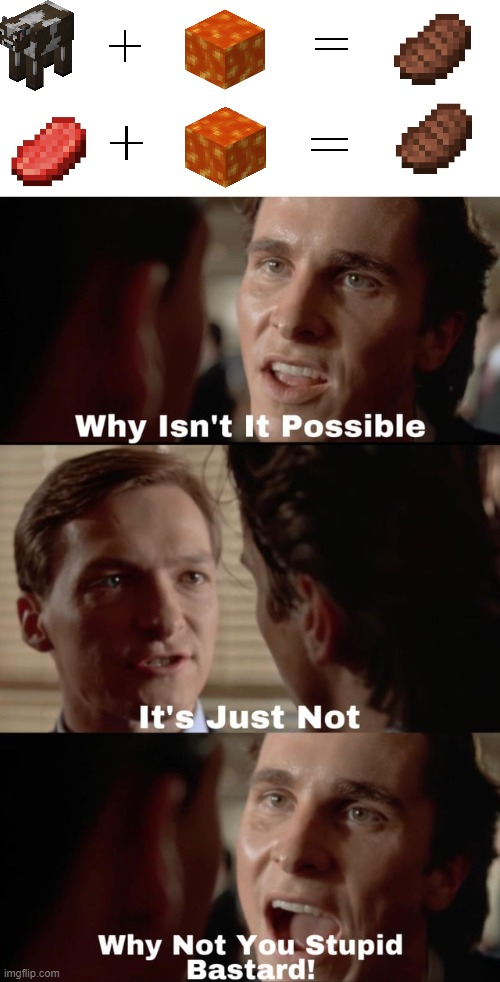
\includegraphics[scale=0.5]{fun_img/img1.jpg}\caption{График функции $u^2(T)$.}\end{figure}\begin{equation*}
\begin{wrapeqn}
 f(x) = \cos {x}\end{wrapeqn}
\end{equation*}
Методом введения ЛСД в вену получили:\newline
\begin{equation*}
\begin{wrapeqn}
f^{1}(x) = -1 \cdot \sin {x}\end{wrapeqn}
\end{equation*}
$$f^{1}(0) = -0$$Методом введения ЛСД в вену получили:\newline
\begin{equation*}
\begin{wrapeqn}
f^{2}(x) = -1 \cdot \cos {x}\end{wrapeqn}
\end{equation*}
$$f^{2}(0) = -1$$Методом введения ЛСД в вену получили:\newline
\begin{equation*}
\begin{wrapeqn}
f^{3}(x) = -1 \cdot -1 \cdot \sin {x}\end{wrapeqn}
\end{equation*}
$$f^{3}(0) = 0$$Сунул в попу я огурчик, выпил скотч и пукнул в стульчик...\newline
A потом получил:\newline
\begin{equation*}
\begin{wrapeqn}
f^{4}(x) = -1 \cdot -1 \cdot \cos {x}\end{wrapeqn}
\end{equation*}
$$f^{4}(0) = 1$$Ряд Маклорена:\newline
$$f(x) = \frac{1}{1} +\frac{-1}{2} \cdot x^{2} +\frac{1}{24} \cdot x^{4} +O(x^5)$$
\end{document}